\documentclass{beamer}

%\usepackage[table]{xcolor}
\mode<presentation> {
  \usetheme{Boadilla}
%  \usetheme{Pittsburgh}
%\usefonttheme[2]{sans}
\renewcommand{\familydefault}{cmss}
%\usepackage{lmodern}
%\usepackage[T1]{fontenc}
%\usepackage{palatino}
%\usepackage{cmbright}
  \setbeamercovered{transparent}
\useinnertheme{rectangles}
}
%\usepackage{normalem}{ulem}
%\usepackage{colortbl, textcomp}
\setbeamercolor{normal text}{fg=black}
\setbeamercolor{structure}{fg= black}
\definecolor{trial}{cmyk}{1,0,0, 0}
\definecolor{trial2}{cmyk}{0.00,0,1, 0}
\definecolor{darkgreen}{rgb}{0,.4, 0.1}
\usepackage{array}
\beamertemplatesolidbackgroundcolor{white}  \setbeamercolor{alerted
text}{fg=red}

\setbeamertemplate{caption}[numbered]\newcounter{mylastframe}

%\usepackage{color}
\usepackage{tikz}
\usetikzlibrary{arrows}
\usepackage{colortbl}
%\usepackage[usenames, dvipsnames]{color}
%\setbeamertemplate{caption}[numbered]\newcounter{mylastframe}c
%\newcolumntype{Y}{\columncolor[cmyk]{0, 0, 1, 0}\raggedright}
%\newcolumntype{C}{\columncolor[cmyk]{1, 0, 0, 0}\raggedright}
%\newcolumntype{G}{\columncolor[rgb]{0, 1, 0}\raggedright}
%\newcolumntype{R}{\columncolor[rgb]{1, 0, 0}\raggedright}

%\begin{beamerboxesrounded}[upper=uppercol,lower=lowercol,shadow=true]{Block}
%$A = B$.
%\end{beamerboxesrounded}}
\renewcommand{\familydefault}{cmss}
%\usepackage[all]{xy}

\usepackage{tikz}
\usepackage{lipsum}

 \newenvironment{changemargin}[3]{%
 \begin{list}{}{%
 \setlength{\topsep}{0pt}%
 \setlength{\leftmargin}{#1}%
 \setlength{\rightmargin}{#2}%
 \setlength{\topmargin}{#3}%
 \setlength{\listparindent}{\parindent}%
 \setlength{\itemindent}{\parindent}%
 \setlength{\parsep}{\parskip}%
 }%
\item[]}{\end{list}}
\usetikzlibrary{arrows}
%\usepackage{palatino}
%\usepackage{eulervm}
\usecolortheme{lily}
\newtheorem{com}{Comment}
\newtheorem{lem} {Lemma}
\newtheorem{prop}{Proposition}
\newtheorem{thm}{Theorem}
\newtheorem{defn}{Definition}
\newtheorem{cor}{Corollary}
\newtheorem{obs}{Observation}
 \numberwithin{equation}{section}
%\usepackage[latin1]{inputenc}
\title[Machine Learning] % (optional, nur bei langen Titeln nötig)
{Machine Learning}

\author{Justin Grimmer}
\institute[University of Chicago]{Associate Professor\\Department of Political Science \\  University of Chicago}
\vspace{0.3in}


\date{February 21st, 2018}%[Big Data Workshop]
%\date{\today}




\begin{document}
\begin{frame}
\titlepage
\end{frame}



\begin{frame}

\huge

Measurement via repurposed discovery methods
\begin{itemize}
\item[1)] Discovery categories, measure prevalence of categories
\item[2)] Once we fix \alert{interpretation}, accuracy/precision/recall well defined
\end{itemize}	


\end{frame}




\begin{frame}
\frametitle{LDA Revisited}


\only<1>{\begin{eqnarray}
\boldsymbol{\theta}_{k} & \sim & \text{Dirichlet}(\boldsymbol{1}) \nonumber \\
\boldsymbol{\pi}_{i}|\boldsymbol{\alpha} & \sim &  \text{Dirichlet}(\boldsymbol{\alpha}) \nonumber \\
\boldsymbol{\tau}_{im}| \boldsymbol{\pi}_{i} & \sim & \text{Multinomial}(1, \boldsymbol{\pi}_{i}) \nonumber \\
x_{im} | \boldsymbol{\theta}_{k}, \tau_{imk} = 1 & \sim & \text{Multinomial}(1, \boldsymbol{\theta}_{k}) \nonumber
\end{eqnarray}}

\only<2>{\begin{eqnarray}
\textbf{Unigram Model}_{k} & \sim & \text{Dirichlet}(\boldsymbol{1}) \nonumber \\
\textbf{Doc. Prop}_{i} & \sim & \text{Dirichlet}(\textbf{Pop. Proportion}) \nonumber \\
\textbf{Word Topic}_{im} & \sim & \text{Multinomial}(1, \textbf{Doc. Prop}_{i}) \nonumber \\
\text{Word}_{im} & \sim & \text{Multinomial}(1, \textbf{Unigram Model}_{k}) \nonumber
\end{eqnarray}}







\end{frame}



\begin{frame}
\frametitle{A General Hierarchical Structure}

LDA:
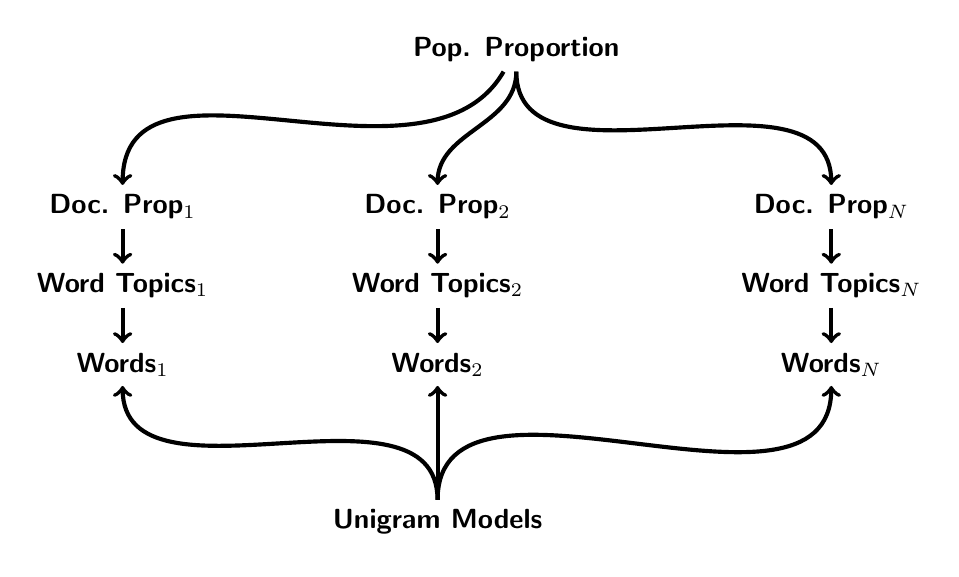
\begin{tikzpicture}

\node (col) at (0, 10) [] {\textbf{Pop. Proportion}} ;

\invisible<1>{



\node (doc1) at (-5, 8) [] {\textbf{Doc. Prop}$_{1}$} ;
\node (doc2) at (-1, 8) [] {\textbf{Doc. Prop}$_{2}$} ;
\node (dots) at ( 2, 8) [] {$\hdots$} ;
\node (docN) at (4, 8) [] {\textbf{Doc. Prop}$_{N}$} ;

\draw[->, line width=1.5pt] (col) to [out=240, in = 90] (doc1);
\draw[->, line width=1.5pt] (col) to [out=270, in = 90] (doc2);
\draw[->, line width=1.5pt] (col) to [out=270, in = 90] (docN);

}

\invisible<1-2>{


\node (word11) at (-5, 7) [] {\textbf{Word Topics}$_{1}$} ;
\node (word22) at (-1, 7) [] {\textbf{Word Topics}$_{2}$} ;
\node (wordnn) at (4, 7) [] {\textbf{Word Topics}$_{N}$ } ;

\draw[->, line width=1.5pt] (doc1) to [out=270, in=90] (word11) ;
\draw[->, line width=1.5pt] (doc2) to [out=270, in=90] (word22) ;
\draw[->, line width=1.5pt] (docN) to [out=270, in=90] (wordnn) ;




}



\invisible<1-3>{

\node (wordaa) at (-5, 6) [] {\textbf{Words}$_{1}$} ;
\node (wordbb) at (-1, 6) [] {\textbf{Words}$_{2}$} ;
\node (wordcc) at (4, 6) [] {\textbf{Words}$_{N}$ } ;


\draw[->, line width = 1.5pt] (word11) to [out = 270, in = 90] (wordaa);
\draw[->, line width = 1.5pt] (word22) to [out = 270, in = 90] (wordbb);
\draw[->, line width = 1.5pt] (wordnn) to [out = 270, in = 90] (wordcc);

\node (topics) at (-1, 4) [] {$\textbf{Unigram Models}$} ;



\draw[->, line width = 1.5pt] (topics) to [out = 90, in = 270] (wordaa);
\draw[->, line width = 1.5pt] (topics) to [out = 90, in = 270] (wordbb);
\draw[->, line width = 1.5pt] (topics) to [out = 90, in = 270] (wordcc);



}


\end{tikzpicture}


\pause \pause \pause

\end{frame}



\begin{frame}
\frametitle{A General Hierarchical Structure}

Dynamic Topic Model (Quinn et al 2010)
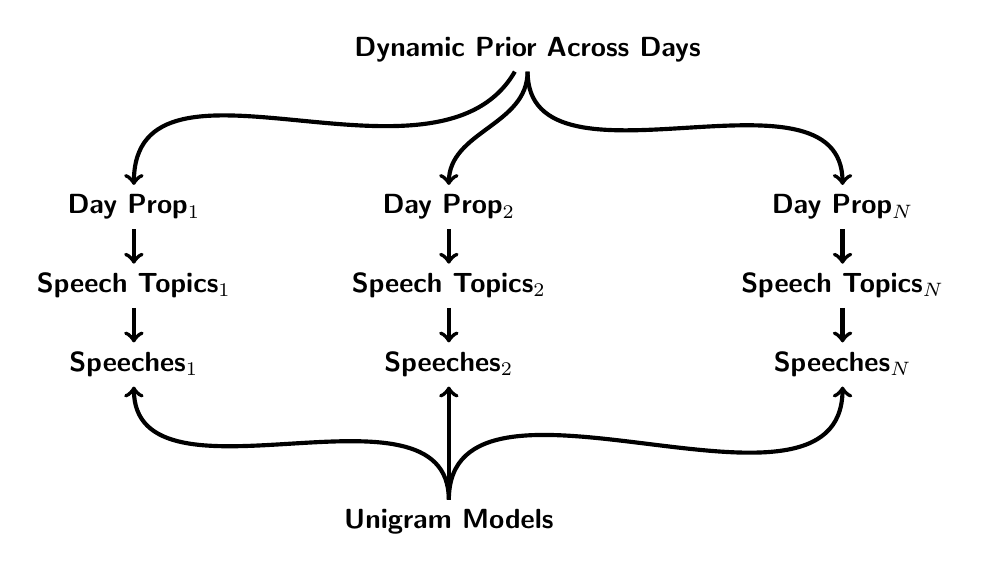
\begin{tikzpicture}

\node (col) at (0, 10) [] {\textbf{Dynamic Prior Across Days}} ;

\invisible<1>{



\node (doc1) at (-5, 8) [] {\textbf{Day Prop}$_{1}$} ;
\node (doc2) at (-1, 8) [] {\textbf{Day Prop}$_{2}$} ;
\node (dots) at ( 2, 8) [] {$\hdots$} ;
\node (docN) at (4, 8) [] {\textbf{Day Prop}$_{N}$} ;

\draw[->, line width=1.5pt] (col) to [out=240, in = 90] (doc1);
\draw[->, line width=1.5pt] (col) to [out=270, in = 90] (doc2);
\draw[->, line width=1.5pt] (col) to [out=270, in = 90] (docN);

}

\invisible<1-2>{


\node (word11) at (-5, 7) [] {\textbf{Speech Topics}$_{1}$} ;
\node (word22) at (-1, 7) [] {\textbf{Speech Topics}$_{2}$} ;
\node (wordnn) at (4, 7) [] {\textbf{Speech Topics}$_{N}$ } ;

\draw[->, line width=1.5pt] (doc1) to [out=270, in=90] (word11) ;
\draw[->, line width=1.5pt] (doc2) to [out=270, in=90] (word22) ;
\draw[->, line width=1.5pt] (docN) to [out=270, in=90] (wordnn) ;




}



\invisible<1-3>{

\node (wordaa) at (-5, 6) [] {\textbf{Speeches}$_{1}$} ;
\node (wordbb) at (-1, 6) [] {\textbf{Speeches}$_{2}$} ;
\node (wordcc) at (4, 6) [] {\textbf{Speeches}$_{N}$ } ;


\draw[->, line width = 1.5pt] (word11) to [out = 270, in = 90] (wordaa);
\draw[->, line width = 1.5pt] (word22) to [out = 270, in = 90] (wordbb);
\draw[->, line width = 1.5pt] (wordnn) to [out = 270, in = 90] (wordcc);

\node (topics) at (-1, 4) [] {$\textbf{Unigram Models}$} ;



\draw[->, line width = 1.5pt] (topics) to [out = 90, in = 270] (wordaa);
\draw[->, line width = 1.5pt] (topics) to [out = 90, in = 270] (wordbb);
\draw[->, line width = 1.5pt] (topics) to [out = 90, in = 270] (wordcc);



}


\end{tikzpicture}


\pause \pause \pause

\end{frame}




\begin{frame}
\frametitle{A General Hierarchical Structure}

Expressed Agenda Model (Grimmer 2010)
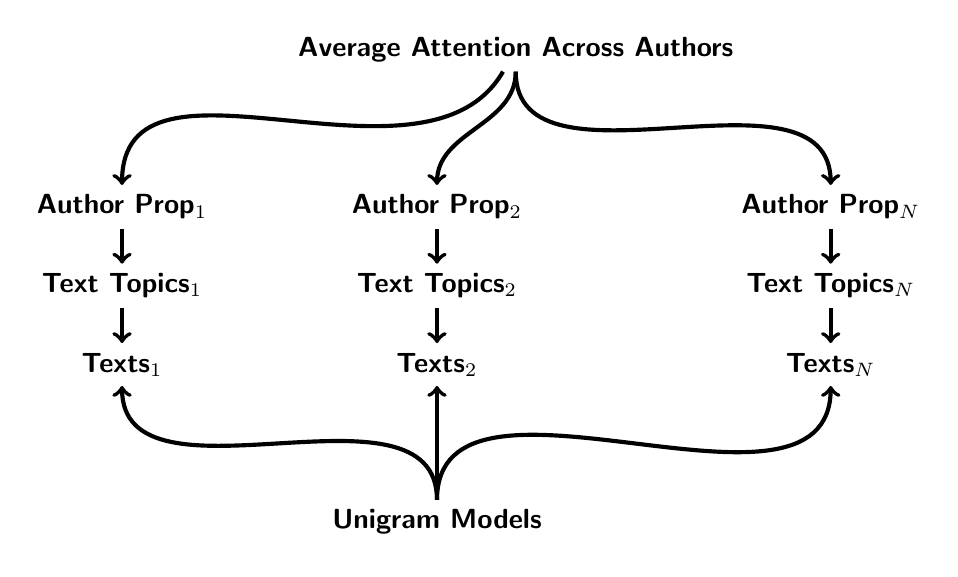
\begin{tikzpicture}

\node (col) at (0, 10) [] {\textbf{Average Attention Across Authors}} ;

\invisible<1>{



\node (doc1) at (-5, 8) [] {\textbf{Author Prop}$_{1}$} ;
\node (doc2) at (-1, 8) [] {\textbf{Author Prop}$_{2}$} ;
\node (dots) at ( 2, 8) [] {$\hdots$} ;
\node (docN) at (4, 8) [] {\textbf{Author Prop}$_{N}$} ;

\draw[->, line width=1.5pt] (col) to [out=240, in = 90] (doc1);
\draw[->, line width=1.5pt] (col) to [out=270, in = 90] (doc2);
\draw[->, line width=1.5pt] (col) to [out=270, in = 90] (docN);

}

\invisible<1-2>{


\node (word11) at (-5, 7) [] {\textbf{Text Topics}$_{1}$} ;
\node (word22) at (-1, 7) [] {\textbf{Text Topics}$_{2}$} ;
\node (wordnn) at (4, 7) [] {\textbf{Text Topics}$_{N}$ } ;

\draw[->, line width=1.5pt] (doc1) to [out=270, in=90] (word11) ;
\draw[->, line width=1.5pt] (doc2) to [out=270, in=90] (word22) ;
\draw[->, line width=1.5pt] (docN) to [out=270, in=90] (wordnn) ;




}



\invisible<1-3>{

\node (wordaa) at (-5, 6) [] {\textbf{Texts}$_{1}$} ;
\node (wordbb) at (-1, 6) [] {\textbf{Texts}$_{2}$} ;
\node (wordcc) at (4, 6) [] {\textbf{Texts}$_{N}$ } ;


\draw[->, line width = 1.5pt] (word11) to [out = 270, in = 90] (wordaa);
\draw[->, line width = 1.5pt] (word22) to [out = 270, in = 90] (wordbb);
\draw[->, line width = 1.5pt] (wordnn) to [out = 270, in = 90] (wordcc);

\node (topics) at (-1, 4) [] {$\textbf{Unigram Models}$} ;



\draw[->, line width = 1.5pt] (topics) to [out = 90, in = 270] (wordaa);
\draw[->, line width = 1.5pt] (topics) to [out = 90, in = 270] (wordbb);
\draw[->, line width = 1.5pt] (topics) to [out = 90, in = 270] (wordcc);



}


\end{tikzpicture}


\pause \pause \pause

\end{frame}


\begin{frame}
\frametitle{A General Hierarchical Structure}

Structural Topic Model (Roberts, Stewart, Airoldi 2014)
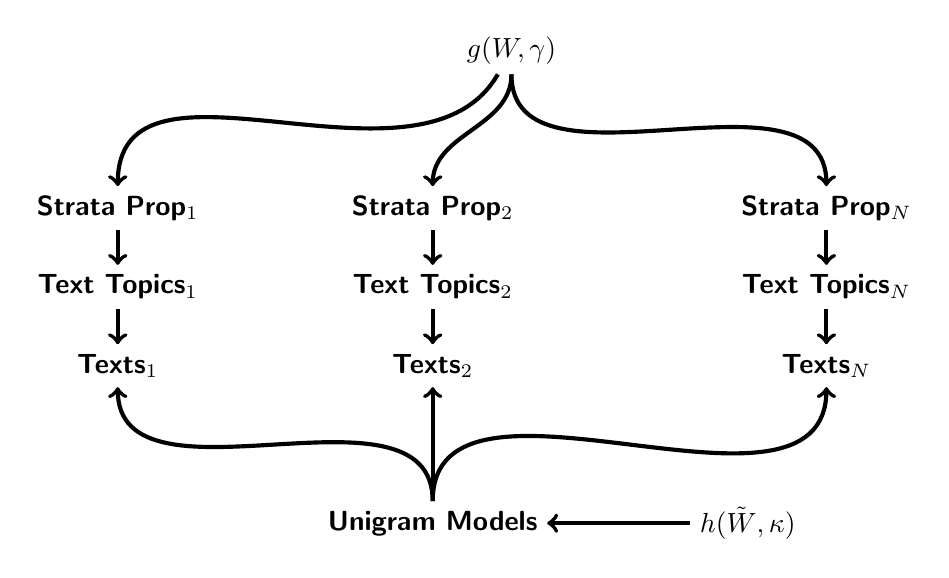
\begin{tikzpicture}

\node (col) at (0, 10) [] {$g(\boldsymbol{W}, \boldsymbol{\gamma}) $} ;

\invisible<1>{



\node (doc1) at (-5, 8) [] {\textbf{Strata Prop}$_{1}$} ;
\node (doc2) at (-1, 8) [] {\textbf{Strata Prop}$_{2}$} ;
\node (dots) at ( 2, 8) [] {$\hdots$} ;
\node (docN) at (4, 8) [] {\textbf{Strata Prop}$_{N}$} ;

\draw[->, line width=1.5pt] (col) to [out=240, in = 90] (doc1);
\draw[->, line width=1.5pt] (col) to [out=270, in = 90] (doc2);
\draw[->, line width=1.5pt] (col) to [out=270, in = 90] (docN);

}

\invisible<1-2>{


\node (word11) at (-5, 7) [] {\textbf{Text Topics}$_{1}$} ;
\node (word22) at (-1, 7) [] {\textbf{Text Topics}$_{2}$} ;
\node (wordnn) at (4, 7) [] {\textbf{Text Topics}$_{N}$ } ;

\draw[->, line width=1.5pt] (doc1) to [out=270, in=90] (word11) ;
\draw[->, line width=1.5pt] (doc2) to [out=270, in=90] (word22) ;
\draw[->, line width=1.5pt] (docN) to [out=270, in=90] (wordnn) ;




}



\invisible<1-3>{

\node (wordaa) at (-5, 6) [] {\textbf{Texts}$_{1}$} ;
\node (wordbb) at (-1, 6) [] {\textbf{Texts}$_{2}$} ;
\node (wordcc) at (4, 6) [] {\textbf{Texts}$_{N}$ } ;


\draw[->, line width = 1.5pt] (word11) to [out = 270, in = 90] (wordaa);
\draw[->, line width = 1.5pt] (word22) to [out = 270, in = 90] (wordbb);
\draw[->, line width = 1.5pt] (wordnn) to [out = 270, in = 90] (wordcc);

\node (topics) at (-1, 4) [] {$\textbf{Unigram Models}$} ;



\draw[->, line width = 1.5pt] (topics) to [out = 90, in = 270] (wordaa);
\draw[->, line width = 1.5pt] (topics) to [out = 90, in = 270] (wordbb);
\draw[->, line width = 1.5pt] (topics) to [out = 90, in = 270] (wordcc);



}

\invisible<1-4>{
\node (reg) at (3, 4) [] {$h(\tilde{\boldsymbol{W}}, \boldsymbol{\kappa})$ };

\draw[->, line width = 1.5pt] (reg) to [out = 180, in = 0] (topics);

}
\end{tikzpicture}


\pause \pause \pause \pause

\end{frame}


\begin{frame}

{\tt R Code}


\end{frame}



\begin{frame}
\frametitle{A General Hierarchical Structure}

Conditioning on Unknown Covariates$\leadsto$ levels of mixtures at proportions (Grimmer 2013; Wallach 2008)
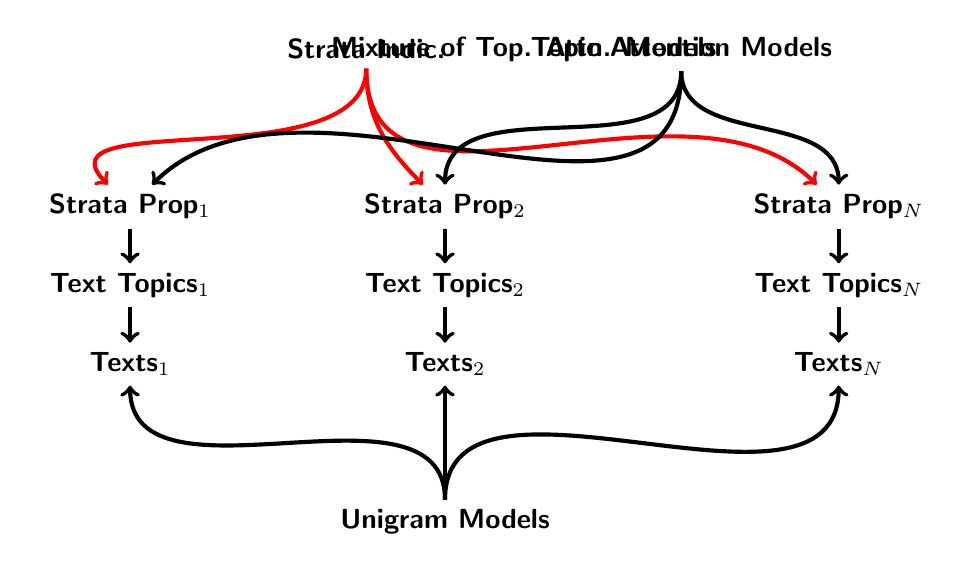
\begin{tikzpicture}

\only<1>{\node (col_on) at (0, 10)[] {\textbf{Mixture of Top. Attn. Models}} ; }

\invisible<1>{\node (col1) at (-2, 10) [] {\textbf{Strata Indic.} } ;
\node (col) at (2, 10) [] {\textbf{Topic Attention Models} }  ; }

\invisible<1-2>{



\node (doc1) at (-5, 8) [] {\textbf{Strata Prop}$_{1}$} ;
\node (doc2) at (-1, 8) [] {\textbf{Strata Prop}$_{2}$} ;
\node (dots) at ( 2, 8) [] {$\hdots$} ;
\node (docN) at (4, 8) [] {\textbf{Strata Prop}$_{N}$} ;


\draw[->, line width=1.5pt, red] (col1) to [out=270, in = 135] (doc1);
\draw[->, line width=1.5pt, red] (col1) to [out=270, in = 135] (doc2);
\draw[->, line width=1.5pt, red] (col1) to [out=270, in = 135] (docN);
}

\invisible<1-3>{

\draw[->, line width=1.5pt] (col) to [out=270, in = 45] (doc1);
\draw[->, line width=1.5pt] (col) to [out=270, in = 90] (doc2);
\draw[->, line width=1.5pt] (col) to [out=270, in = 90] (docN);




}

\invisible<1-4>{


\node (word11) at (-5, 7) [] {\textbf{Text Topics}$_{1}$} ;
\node (word22) at (-1, 7) [] {\textbf{Text Topics}$_{2}$} ;
\node (wordnn) at (4, 7) [] {\textbf{Text Topics}$_{N}$ } ;

\draw[->, line width=1.5pt] (doc1) to [out=270, in=90] (word11) ;
\draw[->, line width=1.5pt] (doc2) to [out=270, in=90] (word22) ;
\draw[->, line width=1.5pt] (docN) to [out=270, in=90] (wordnn) ;




}



\invisible<1-5>{

\node (wordaa) at (-5, 6) [] {\textbf{Texts}$_{1}$} ;
\node (wordbb) at (-1, 6) [] {\textbf{Texts}$_{2}$} ;
\node (wordcc) at (4, 6) [] {\textbf{Texts}$_{N}$ } ;


\draw[->, line width = 1.5pt] (word11) to [out = 270, in = 90] (wordaa);
\draw[->, line width = 1.5pt] (word22) to [out = 270, in = 90] (wordbb);
\draw[->, line width = 1.5pt] (wordnn) to [out = 270, in = 90] (wordcc);

\node (topics) at (-1, 4) [] {$\textbf{Unigram Models}$} ;



\draw[->, line width = 1.5pt] (topics) to [out = 90, in = 270] (wordaa);
\draw[->, line width = 1.5pt] (topics) to [out = 90, in = 270] (wordbb);
\draw[->, line width = 1.5pt] (topics) to [out = 90, in = 270] (wordcc);



}


\end{tikzpicture}


\pause \pause \pause \pause \pause

\end{frame}



\begin{frame}
\frametitle{A General Hierarchical Structure}

Conditioning on Unknown Covariates for Topics$\leadsto$ hierarchy of topics (Li and McCallum 2006; Blaydes, Grimmer, and McQueen 2017)
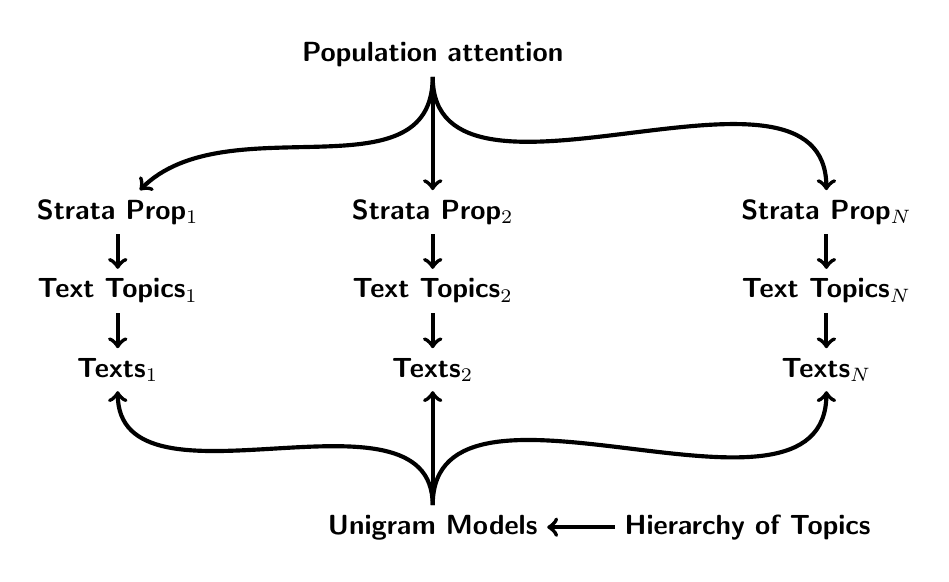
\begin{tikzpicture}

\node (col) at (-1, 10)[] {\textbf{Population attention}} ;

\invisible<1>{



\node (doc1) at (-5, 8) [] {\textbf{Strata Prop}$_{1}$} ;
\node (doc2) at (-1, 8) [] {\textbf{Strata Prop}$_{2}$} ;
\node (dots) at ( 2, 8) [] {$\hdots$} ;
\node (docN) at (4, 8) [] {\textbf{Strata Prop}$_{N}$} ;



\draw[->, line width=1.5pt] (col) to [out=270, in = 45] (doc1);
\draw[->, line width=1.5pt] (col) to [out=270, in = 90] (doc2);
\draw[->, line width=1.5pt] (col) to [out=270, in = 90] (docN);




}

\invisible<1-2>{


\node (word11) at (-5, 7) [] {\textbf{Text Topics}$_{1}$} ;
\node (word22) at (-1, 7) [] {\textbf{Text Topics}$_{2}$} ;
\node (wordnn) at (4, 7) [] {\textbf{Text Topics}$_{N}$ } ;

\draw[->, line width=1.5pt] (doc1) to [out=270, in=90] (word11) ;
\draw[->, line width=1.5pt] (doc2) to [out=270, in=90] (word22) ;
\draw[->, line width=1.5pt] (docN) to [out=270, in=90] (wordnn) ;




}



\invisible<1-3>{

\node (wordaa) at (-5, 6) [] {\textbf{Texts}$_{1}$} ;
\node (wordbb) at (-1, 6) [] {\textbf{Texts}$_{2}$} ;
\node (wordcc) at (4, 6) [] {\textbf{Texts}$_{N}$ } ;


\draw[->, line width = 1.5pt] (word11) to [out = 270, in = 90] (wordaa);
\draw[->, line width = 1.5pt] (word22) to [out = 270, in = 90] (wordbb);
\draw[->, line width = 1.5pt] (wordnn) to [out = 270, in = 90] (wordcc);

\node (topics) at (-1, 4) [] {$\textbf{Unigram Models}$} ;



\draw[->, line width = 1.5pt] (topics) to [out = 90, in = 270] (wordaa);
\draw[->, line width = 1.5pt] (topics) to [out = 90, in = 270] (wordbb);
\draw[->, line width = 1.5pt] (topics) to [out = 90, in = 270] (wordcc);



}

\invisible<1-4>{
\node (mix) at (3, 4) [] {\textbf{Hierarchy of Topics}} ;
\draw[->, line width = 1.5pt] (mix) to [out = 180, in = 0] (topics);
}


\end{tikzpicture}


\pause \pause \pause \pause \pause

\end{frame}

\begin{frame}
\frametitle{Why Encode Structure in Extensions of LDA?}

\pause

\begin{itemize}
\invisible<1>{\item[-] Substantive reasons} \pause
\begin{itemize}
\invisible<1-2>{\item[-] Additional structure corresponds to substantively interesting content} \pause
\invisible<1-3>{\item[-] Avoids potential ad-hoc secondary analysis} \pause
\invisible<1-4>{\item[-] Clear data generating process} \pause
\end{itemize}
\invisible<1-5>{\item[-] Statistical reasons} \pause
\begin{itemize}
\invisible<1-6>{\item[-] \alert{Smoothing}$\leadsto$ borrow information across groups intelligently} \pause
\invisible<1-7>{\item[-] \alert{Uncertainty}$\leadsto$ potential for better uncertainty estimates} \pause
\invisible<1-8>{\item[-] \alert{Improved topics}$\leadsto$ small word conditions, structure could help}
\end{itemize}
\end{itemize}





\end{frame}




\begin{frame}
\frametitle{Plan for the Class}

\begin{itemize}
\item[1)] Discuss model with unknown covariates for strata proportions$\leadsto$ presentational style
\item[2)] Discuss model with hierarchy of topics$\leadsto$ mirrors genre
\end{itemize}


\end{frame}



\begin{frame}
\frametitle{Unknown Covariates for Issue Attention: Measuring Attention in Senate Press Releases}

Substantive problem: \pause  \\
\invisible<1>{Senators (representatives) regularly engage the public $\rightarrow$ presentational style\\
But we know little about this engagement} \pause \\
\invisible<1-2>{Why?  \alert{Hard to Measure} } \pause \\

\invisible<1-3>{Describe model that facilitates estimation of \alert{presentational styles} in Senate press releases} \pause
\begin{itemize}
\invisible<1-4>{\item[-] Characterize representation provided to constituents} \pause
\invisible<1-5>{\item[-] Divide attention over a set of topics} \pause
\invisible<1-6>{\item[-] Given attention to topics, write press releases}
\end{itemize}
\end{frame}







\begin{frame}
\frametitle{Presentational Styles$\leadsto$ Objective Function}
\begin{itemize}
\item[-] $\pi_{itk} \equiv$ Attention senator $i$ allocates to
issue $k$ in year $t$
\item[-] $\pi_{itk} \equiv$ Probability press release is
about issue $k$
\item[-] $\boldsymbol{\pi}_{it} = (\pi_{it1},
\hdots, \pi_{it 44}) $
\end{itemize}
\pause
\invisible<1>{Press release-level parameters (press release $j$ from senator $i$
in year $t$)} \pause
\begin{itemize}
\invisible<1-2>{\item[-] \alert{Assume}: Each press release $j$
assigned to one topic.
\item[-] Let
$\boldsymbol{\tau}_{ijt}$ indicate press release $j$'s topic.} \pause
\end{itemize}
\invisible<1-3>{\begin{center} $\boldsymbol{\tau}_{ijt} \sim
\text{Multinomial}(1, \boldsymbol{\pi}_{it}) $ \end{center}} \pause
\begin{itemize}
\invisible<1-4>{\item[-] Conditional on topic, draw document's
content.} \pause
\invisible<1-5>{\item[-] If $\tau_{ijtk} =1$ then
\end{itemize}
\begin{center}$\boldsymbol{x}_{ijt} \sim \text{Multinomial}(n_{ijt}, \boldsymbol{\theta}_k
).$}
\end{center}
\end{frame}

\begin{frame}
\frametitle{Priors}

 Each $\boldsymbol{\pi}_{it}$ is a draw from one-of-$S$ styles$\leadsto$ mixture of Dirichlet distributions \pause .
\begin{eqnarray}
 \invisible<1>{\boldsymbol{\sigma}_{it} & \sim  & \text{Multinomial}(1, \boldsymbol{\beta}). } \pause \nonumber \\
 \invisible<1-2>{\boldsymbol{\pi}_{it}|\sigma_{its}=1, \boldsymbol{\alpha}_s & \sim &  \text{Dirichlet}(\boldsymbol{\alpha}_s) \nonumber } \pause \\
\invisible<1-3>{\alpha_{ks} & \sim & \text{Gamma}(0.25, 1)} \pause  \nonumber
\end{eqnarray}

\invisible<1-4>{Other priors:} \pause
\begin{eqnarray}
\invisible<1-5>{\boldsymbol{\theta}_k & \sim & \text{Multinomial}(\boldsymbol{\lambda}) \nonumber \\} \pause
\invisible<1-6>{\boldsymbol{\beta} & \sim & \text{Multinomial}(\boldsymbol{1})}
\nonumber
\end{eqnarray}

\end{frame}



%\begin{frame}
%\begin{eqnarray}
%\alpha_{sk} & \sim & \text{Gamma}(0.25, 1) \text{ for all } k, s \nonumber \\
%\boldsymbol{\beta} & \sim & \text{Dirichlet}(\boldsymbol{1}) \nonumber \\
%\boldsymbol{\theta}_k & \sim & \text{Dirichlet}(\boldsymbol{\lambda} ) \nonumber \\
%\boldsymbol{\sigma}_{it} | \boldsymbol{\beta} & \sim & \text{Multinomial}(1, \boldsymbol{\beta} ) \text{ for all } i ; t \nonumber \\
%\boldsymbol{\pi}_{it} | \boldsymbol{\sigma}_{its}=1, \boldsymbol{\alpha}_s & \sim & \text{Dirichlet}(\boldsymbol{\alpha}_s) \text{ for all } i ; t  \nonumber \\
%\boldsymbol{\tau}_{ijt}|\boldsymbol{\pi}_{it} & \sim & \text{Multinomial}(1, \boldsymbol{\pi}_{it} ) \text{ for all } j ; t ; i  \nonumber \\
%\boldsymbol{y}_{ijt} | \boldsymbol{\tau}_{ijtk} = 1,
%\boldsymbol{\theta}_k & \sim & \text{Multinomial}(n_{ijt},
%\boldsymbol{\theta}_k) \text{ for all } j ; t ; i  \nonumber
%\end{eqnarray}
%\end{frame}


\begin{frame}
\frametitle{Presentational Styles$\leadsto$ Objective Function}

\pause
\begin{eqnarray}
\invisible<1>{\boldsymbol{\beta}& \sim & \text{Dirichlet}(\boldsymbol{1}) \nonumber } \\
\invisible<1>{\boldsymbol{\theta}_{k} & \sim & \text{Dirichlet}(\boldsymbol{\lambda}) \nonumber}  \\
\invisible<1>{\alpha_{ks} & \sim & \text{Gamma}(0.25, 1) \nonumber}  \\
\invisible<1-2>{\boldsymbol{\sigma}_{it} & \sim & \text{Multinomial}(1, \boldsymbol{\beta}) \nonumber } \\
\invisible<1-3>{\boldsymbol{\pi}_{it}| \sigma_{its} = 1, \boldsymbol{\alpha}_{s} & \sim & \text{Dirichlet}(\boldsymbol{\alpha}_{s})\nonumber} \\
\invisible<1-4>{\boldsymbol{\tau}_{ijt} | \boldsymbol{\pi}_{it} & \sim & \text{Multinomial}(1, \boldsymbol{\pi}_{it}) \nonumber \\}
\invisible<1-5>{\boldsymbol{x}_{ijt}| \tau_{ijtk} = 1, \boldsymbol{\theta}_{k} & \sim & \text{Multinomial}(n_{ijt}, \boldsymbol{\theta}_{k})\nonumber }
\end{eqnarray}


\pause \pause \pause \pause \pause
\end{frame}


\begin{frame}
\frametitle{Mixture of Styles, Mixture of Topics}

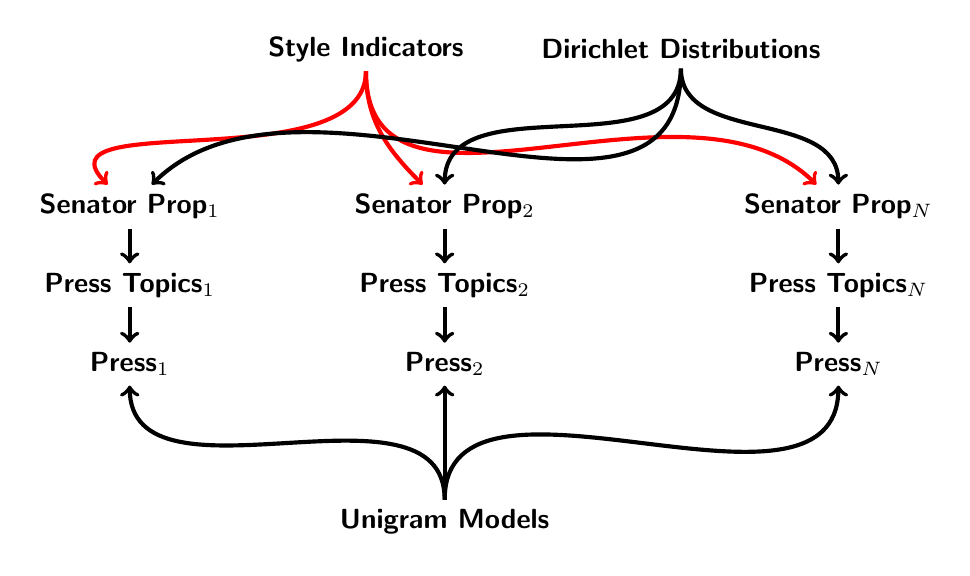
\begin{tikzpicture}

\node (col1) at (-2, 10) [] {\textbf{Style Indicators} } ;
\node (col) at (2, 10) [] {\textbf{Dirichlet Distributions} }  ;




\node (doc1) at (-5, 8) [] {\textbf{Senator Prop}$_{1}$} ;
\node (doc2) at (-1, 8) [] {\textbf{Senator Prop}$_{2}$} ;
\node (dots) at ( 2, 8) [] {$\hdots$} ;
\node (docN) at (4, 8) [] {\textbf{Senator Prop}$_{N}$} ;


\draw[->, line width=1.5pt, red] (col1) to [out=270, in = 135] (doc1);
\draw[->, line width=1.5pt, red] (col1) to [out=270, in = 135] (doc2);
\draw[->, line width=1.5pt, red] (col1) to [out=270, in = 135] (docN);



\draw[->, line width=1.5pt] (col) to [out=270, in = 45] (doc1);
\draw[->, line width=1.5pt] (col) to [out=270, in = 90] (doc2);
\draw[->, line width=1.5pt] (col) to [out=270, in = 90] (docN);





\node (word11) at (-5, 7) [] {\textbf{Press Topics}$_{1}$} ;
\node (word22) at (-1, 7) [] {\textbf{Press Topics}$_{2}$} ;
\node (wordnn) at (4, 7) [] {\textbf{Press Topics}$_{N}$ } ;

\draw[->, line width=1.5pt] (doc1) to [out=270, in=90] (word11) ;
\draw[->, line width=1.5pt] (doc2) to [out=270, in=90] (word22) ;
\draw[->, line width=1.5pt] (docN) to [out=270, in=90] (wordnn) ;



\node (wordaa) at (-5, 6) [] {\textbf{Press}$_{1}$} ;
\node (wordbb) at (-1, 6) [] {\textbf{Press}$_{2}$} ;
\node (wordcc) at (4, 6) [] {\textbf{Press}$_{N}$ } ;


\draw[->, line width = 1.5pt] (word11) to [out = 270, in = 90] (wordaa);
\draw[->, line width = 1.5pt] (word22) to [out = 270, in = 90] (wordbb);
\draw[->, line width = 1.5pt] (wordnn) to [out = 270, in = 90] (wordcc);

\node (topics) at (-1, 4) [] {$\textbf{Unigram Models}$} ;



\draw[->, line width = 1.5pt] (topics) to [out = 90, in = 270] (wordaa);
\draw[->, line width = 1.5pt] (topics) to [out = 90, in = 270] (wordbb);
\draw[->, line width = 1.5pt] (topics) to [out = 90, in = 270] (wordcc);



\end{tikzpicture}



\end{frame}



\begin{frame}

Posterior: \tiny
\begin{eqnarray}
p(\boldsymbol{\alpha}, \boldsymbol{\beta}, \boldsymbol{\theta},
\boldsymbol{\sigma}, \boldsymbol{\pi},
\boldsymbol{\tau}|\boldsymbol{X}) & \propto &
\prod_{k=1}^{K}\prod_{s=1}^{S} \frac{\exp( -
\frac{\alpha_{ks}}{1/4})}{1/4} \times \frac{\Gamma(\sum_{w=1}^{W}
\lambda_w) }{\prod_{w=1}^{W} \Gamma(\lambda_w) } \prod_{w=1}^{W}
\theta_{k,w}^{\lambda_w - 1}
\times \nonumber \\
& & \prod_{i=1}^{N} \prod_{t=2005}^{2007} \prod_{s=1}^{S} \left[
\beta_s \frac{\Gamma(\sum_{k=1}^{K} \alpha_{ks})}{\prod_{k=1}^{K}
\Gamma(\alpha_{ks} )} \prod_{k=1}^{K} \pi_{itk}^{\alpha_{ks}-1}
\prod_{j=1}^{D_{it} }\prod_{k=1}^{K} \left[ \pi_{itk}
\prod_{w=1}^{W} \theta_{kw} ^{x_{ijtw} }
 \right]^{\tau_{ijtk}} \right]^{\sigma_{its}} \nonumber
\end{eqnarray}

\pause


\normalsize
\begin{itemize}
\invisible<1>{\item[1)] Estimate with Variational Approximation} \pause
\invisible<1-2>{\item[2)] Determining number of clusters at top? (Grimmer, Shorey, Wallach, and Zlotnick, In Progress)} \pause
\begin{itemize}
\invisible<1-3>{\item[-] Non-parametric model$\leadsto$ statistical selection} \pause
\invisible<1-4>{\item[-] Experiments/Coding Exercises to assess}
\end{itemize}

\end{itemize}


\end{frame}


\begin{frame}


\only<1>{\scalebox{0.35}{\includegraphics{ShelbyPress.pdf}}}
\only<2>{\scalebox{0.35}{\includegraphics{SessionsPress.pdf}}}




\end{frame}


\begin{frame}
\frametitle{Notions of validity: From Quinn, Monroe, et al (2010) }

\begin{enumerate}
\item[-] \alert{Semantic Validity:} All categories are coherent and meaningful
\item[-] \alert{Convergent Construct Validity:} Measures concur with existing measures in critical details.
\item[-]  \alert{Discriminant Construct Validity}: Measures differ from existing measures in productive ways.
\item[-] \alert{Predictive Measure:} Measures from the model corresponds to external events in expected ways.
\item[-] \alert{Hypothesis Validity:} Measures generated from the model can be used to test substantive hypotheses.
\end{enumerate}

To establish utility of new measures, demonstrate variety of \alert{validations}\\
\alert{None of these validations are performed using a canned statistic}\\
\alert{All}: require substantive knowledge on areas (and what we expect!) [

\end{frame}


\begin{frame}
\frametitle{Home Style Measures, Semantic Validity}


\alert{Must}: Demonstrate to reader that topics are coherent and semantically meaningful

\begin{tabular}{lll}
\hline\hline
Description & Stems & \% \\
\hline
Honorary& honor,prayer,rememb,fund,tribut& 5.0\\
Transp. Grants& airport,transport,announc,urban,hud&4.8\\
Iraq& iraq,iraqi,troop,war,sectarian& 4.7\\
DHS Policy& homeland,port,terrorist,dh,fema&4.1\\
Judicial Nom.& judg,court,suprem,nomin,nomine&3.8\\
Fire Dept. Grant& firefight,homeland,afgp,award,equip&3.7\\
\hline
\end{tabular}

How: \alert{examples} in text are also useful.


\end{frame}


\begin{frame}
\frametitle{Home Style Measures, Convergent Validity}

\only<1-3>{\alert{Over time variation} }
\only<4>{\alert{Supervised/Unsupervised Convergence} }
\only<1>{\scalebox{0.4}{\includegraphics{ImmigrationPlot.pdf}}}
\only<2>{\scalebox{0.4}{\includegraphics{IraqWarPlot.pdf}}}
%\only<3>{\scalebox{0.4}{\includegraphics{Worker5.pdf}}}
\only<3>{\scalebox{0.4}{\includegraphics{HonorPlot.pdf}}}

\only<4>{\scalebox{0.3}{\includegraphics{SupervisedUnsupervised.pdf}}}
\only<5>{\scalebox{0.3}{\includegraphics{ConvValid.pdf}}}

\end{frame}


\begin{frame}
\frametitle{Discriminant Construct Validity}

\scalebox{0.45}{\includegraphics{IdealAttn.pdf} }


\end{frame}



\begin{frame}
\frametitle{Predictive Validity}


\scalebox{0.4}{\includegraphics{CompareLeaders.pdf} }


\end{frame}


\begin{frame}
\frametitle{Hypothesis Validity}


\scalebox{0.28}{\includegraphics{PrioritiesPlotLabel.pdf}}

\begin{columns}[]
\invisible<1>{\column{0.25\textwidth}
\textcolor{blue}{Senate}\\
\textcolor{blue}{Statesperson}
\begin{itemize}
\item[-] \textcolor{blue}{Iraq War}
\item[-] \textcolor{blue}{Intelligence}
\item[-] \textcolor{blue}{Intl. Relations}
\item[-] \textcolor{blue}{Budget}
\end{itemize}}

\invisible<1-2>{\column{0.25\textwidth}
\textcolor{darkgreen}{Domestic}\\
\textcolor{darkgreen}{Policy}
\begin{itemize}
\item[-] \textcolor{darkgreen}{Environment}
\item[-] \textcolor{darkgreen}{Gas prices}
\item[-] \textcolor{darkgreen}{DHS}
\item[-] \textcolor{darkgreen}{Consumer Safety}
\end{itemize}}

\invisible<1-3>{\column{0.25\textwidth} \textcolor{brown}{Pork \&
Policy}
\begin{itemize}
\item[-] \textcolor{brown}{WRDA grants}
\item[-] \textcolor{brown}{Farming}
\item[-] \textcolor{brown}{Health Care}
\item[-] \textcolor{brown}{Education Policy}
\end{itemize}}

\invisible<1-4>{\column{0.25\textwidth}
\textcolor{red}{Appropriators}
\begin{itemize}
\item[-] \textcolor{red}{Fire Grants}
\item[-] \textcolor{red}{Airport Grants}
\item[-] \textcolor{red}{University Money}
\item[-] \textcolor{red}{Police Grants}
\end{itemize}}


\end{columns}

\pause\pause\pause\pause
\end{frame}

\begin{frame}
\frametitle{Hypothesis Validity}


Why do senators adopt different styles?\\
\alert{District Fit}

\scalebox{0.4}{\includegraphics{FinalAvoidance.pdf}}



\end{frame}


\begin{frame}
\frametitle{What are the right number of topics?}

\pause

\begin{itemize}
\invisible<1>{\item[-] Number of topics$\leadsto$ depends on task at hand}
\invisible<1-2>{\item[-] Coarse$\leadsto$ broad comparisons, lose distinctions}
\invisible<1-3>{\item[-] Granular$\leadsto$ specific insights, lose broader picture}
\invisible<1-4>{\item[-] \alert{Hierarchy of topics}$\leadsto$ Pachinko Allocation, Hierarchies of von-Mises Fisher Distributions}
\end{itemize}

\invisible<1-5>{Blaydes, Grimmer, and McQueen 2018$\leadsto$ estimate nested topics to explore the \alert{Mirrors for Princes}}


\pause \pause \pause \pause



\end{frame}




\begin{frame}
\frametitle{The Mirrors Genre (BGM 2017)}


26 Christian mirrors \pause
\begin{itemize}
\invisible<1>{\item[-] The Prince (1513 CE)} \pause
\invisible<1-2>{\item[-] Advice to Justinian (527 CE)} \pause
\invisible<1-3>{\item[-] The Adventures of Telemachus (1699 CE)} \pause
\end{itemize}


\invisible<1-4>{21 Islamic texts} \pause
\begin{itemize}
\invisible<1-5>{\item[-] Advice on the Art of Governance (1612 CE)} \pause
\invisible<1-6>{\item[-] Kalila wa Dimna (748 CE)} \pause
\invisible<1-7>{\item[-] The Sultan's Register of Laws (1632-1633 CE)} \pause
\end{itemize}



\invisible<1-8>{Work with translations}\pause\invisible<1-9>{$\leadsto$ little evidence of selection} \pause
\begin{itemize}
\invisible<1-10>{\item[-] Collect data on collection of 98 (51 Christian, 47 Islamic, some not translated)} \pause
\invisible<1-11>{\item[-] No difference on Year/Region}
\end{itemize}


\end{frame}




\begin{frame}
\frametitle{Preprocessing Texts}

47 books \invisible<1>{$\leadsto$ Each divided into paragraphs} \\
\invisible<1-2>{Create feature space}
\begin{itemize}
\invisible<1-3>{\item[-] Bag of words, stem, discard punctuation, stop words}
\invisible<1-4>{\item[-] Translate words left in Arabic (\alert{allah}) and discard proper nouns}
\invisible<1-5>{\item[-] Identified synonyms}
\begin{itemize}
\invisible<1-6>{\item[-] \alert{almighty}, \alert{god}}
\invisible<1-7>{\item[-] \alert{monarch}, \alert{prince}, \alert{king}, \alert{ruler}}
\invisible<1-8>{\item[-] \alert{Lord} $\neq$ \alert{lord} }
\end{itemize}
\end{itemize}

\invisible<1-9>{Result: short segment $j$ in book $i$ is a count vector}
\begin{eqnarray}
\invisible<1-10>{\textbf{x}_{ij} & = & (x_{ij1}, x_{ij2}, \hdots, x_{ij2124}) \nonumber}
\end{eqnarray}

\invisible<1-11>{We work with a normalized version of the documents, }
\begin{eqnarray}
\invisible<1-12>{\textbf{x}^{*}_{ij} & = & \frac{\textbf{x}_{ij}}{\sqrt{\textbf{x}^{'}_{ij}\textbf{x}_{ij}} } \nonumber}
\end{eqnarray}



\pause \pause \pause \pause \pause \pause \pause \pause \pause \pause \pause \pause


\end{frame}




\begin{frame}
\frametitle{Measuring Themes in the Mirrors}

\only<1-3>{Model built around two hierarchies:
\begin{itemize}
\invisible<1>{\item[1)] Books $\leadsto$ paragraphs (Blei, Ng, Jordan 2003; Wallach, 2008; Quinn et al 2010; Grimmer 2010; Roberts et al 2014)}
\invisible<1-2>{\item[2)] Coarse topics $\leadsto$ granular topics (Li and McCallum 2006; Gopal and Yang 2014)}
\end{itemize}
}


\only<4->{
Estimate \alert{four} quantities of interest
\begin{itemize}
\invisible<1-4>{\item[1)] Granular topics (60)}
\invisible<1-5>{\item[2)] Coarse (broad) topics (3)}
\begin{itemize}
\invisible<1-6>{\item[-] Each granular topic classified into one coarse topic }
\end{itemize}
\invisible<1-7>{\item[3)] Each book $i'$s  $\textbf{themes}_{i}}$
\invisible<1-8>{\item[4)] Each short segment's granular (and coarse) topic }
\end{itemize}




\begin{eqnarray}
\invisible<1-7, 9->{\textbf{themes}_{i} & = & (\text{theme}_{i1}, \text{theme}_{i2}, \hdots, \text{theme}_{i60} ) \nonumber }
\end{eqnarray}

}



\pause \pause \pause \pause \pause \pause \pause \pause
\end{frame}

\begin{frame}
\frametitle{A Hierarchy of Topics}


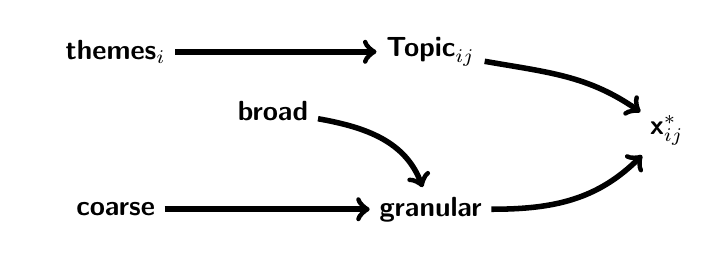
\begin{tikzpicture}

\node (Dummy) at (-9,8) [] {} ;
\node (theme1) at (-8, 9) [] {$\textbf{themes}_{i} $} ;
\invisible<1>{\node (draws) at (-4, 9) [] {$\textbf{Topic}_{ij}$};}
\invisible<1>{\draw[->, line width = 2pt] (theme1) to [out = 0, in = 180] (draws);}

\invisible<1-2>{\node (document) at (-1, 8) [] {$\textbf{x}^{*}_{ij}$ }; }
\invisible<1-2>{\draw[->, line width = 2pt] (draws) to [out = 350, in  = 145] (document); }


\invisible<1-2>{\node (topics)   at (-4, 7) [] {$\textbf{granular}$}; }

\invisible<1-2>{\draw[->, line width = 2pt] (topics) to [out = 0, in = 225] (document) ; }

\invisible<1-3>{\node (topic_sig) at (-6, 8.25) [] {$\textbf{broad}$} ; }

\invisible<1-3>{\draw[->, line width = 2pt] (topic_sig) to [out = 350, in = 110] (topics) ; }

\invisible<1-3>{\node (coarse)    at (-8, 7) [] {$\textbf{coarse}$}; }

\invisible<1-3>{\draw[->, line width = 2pt] (coarse) to [out = 0, in= 180] (topics) ; }

\end{tikzpicture}


\begin{eqnarray}
\invisible<1>{\textbf{Topic}_{ij} & \sim & \text{Multinomial}(1, \textbf{themes}_{i}) \nonumber }\\
\invisible<1-2>{\textbf{x}^{*}_{ij} | \text{Topic}_{ijk} =  1 & \sim & \text{vMF} (\kappa, \textbf{granular}_{k} ) \nonumber }\\
\invisible<1-3>{\textbf{broad}_{k} & \sim & \text{Multinomial}(1, \textbf{Broad Theme Prior}) \nonumber }\\
\invisible<1-3>{\textbf{granular}_{k} | \text{broad}_{km} = 1 & \sim & \text{vMF}(\kappa, \textbf{coarse}_{m}) \nonumber }
\end{eqnarray}

\invisible<1-4>{Estimate model with Variational Approximation}\\
\invisible<1-5>{Model selection: automatic model fit, qualitative evaluation}

\pause \pause \pause \pause \pause




%%draws theme
%%then draws content from a topic specific distribution
%%our model classifies each of those granular themes into coarse themes



\end{frame}





\begin{frame}
\frametitle{Interpreting Unsupervised Models}

Two approaches to labeling output \pause
\begin{itemize}
\invisible<1>{\item[1)] \alert{Computational}: identify discriminating words }\pause
\invisible<1-2>{\item[2)] \alert{Manual}: Segments classified to coarse, granular topics.  Read, discuss, and label} \pause
\end{itemize}

\invisible<1-3>{Unsupervised models \alert{structure} and \alert{guide} our reading}




\end{frame}



\begin{frame}
\frametitle{Art of Rulership}


Practices and ideals of political rule

\vspace{0.5in}
\begin{tabular}{l}
\invisible<1>{king}\invisible<1-2>{,princ}\invisible<1-3>{,citi}\invisible<1-4>{,great,place,work,emperor,enemi,armi,letter} \\
\end{tabular}

\vspace{0.5in}
 \invisible<1-5>{36.5\% of paragraphs }

\pause \pause \pause \pause \pause


\end{frame}

\begin{frame}

\begin{center}
\scalebox{0.45}{\includegraphics{Hist_Super1_p.pdf}}
\end{center}

\end{frame}


\begin{frame}

\begin{center}
\scalebox{0.45}{\includegraphics{Super1.pdf}}
\end{center}


\end{frame}


\begin{frame}
\frametitle{Religion and Virtue}


Connection between religion, virtue, justice and political rule \pause

\vspace{0.5in}
\begin{tabular}{l}
\invisible<1>{almighti,good,virtu,power,ruler,justic,prayer,rule,prophet,mena \\}
\end{tabular}

\pause
\vspace{0.5in}

\invisible<1-2>{32.2\% of pargraphs}

\end{frame}


\begin{frame}

\begin{center}
\scalebox{0.45}{\includegraphics{Hist_Super2_p.pdf}}
\end{center}

\end{frame}



\begin{frame}

\begin{center}
\scalebox{0.45}{\includegraphics{Super2.pdf}}
\end{center}

\end{frame}






\begin{frame}
\frametitle{Inner Life of the Ruler}

Personal relationships, care for and practices of the self, and ultimate fate of the soul \pause

\vspace{0.5in}

\begin{tabular}{ll}
\invisible<1>{man,land,woman,know,bodi,eye,ladi,love,faculti,old} \pause
\end{tabular}

\vspace{0.5in}

\invisible<1-2>{31.2\% of paragraphs}

\end{frame}



\begin{frame}


\begin{center}
\scalebox{0.45}{\includegraphics{Hist_Super3_p.pdf}}
\end{center}

\end{frame}




\begin{frame}

\begin{center}
\scalebox{0.45}{\includegraphics{Super3.pdf}}
\end{center}

\end{frame}



\begin{frame}
\frametitle{Granular: Best Practices for Ruling}


\begin{tabular}{l}
\hline
king,princ,citi,great,place,work,emperor,enemi,armi,letter \\
\hline
\alert{king,kingdom,royal,minist,reign,father,court,majesti,presenc,war}
\end{tabular}

\vspace{0.5in}

6.2\% of paragraphs

\end{frame}



\begin{frame}

\begin{center}
\scalebox{0.45}{\includegraphics{1point1.pdf}}
\end{center}

\end{frame}


\begin{frame}
\frametitle{Granular: Characteristics that distinguish Just Ruler from Tyrant}


\begin{tabular}{l}
\hline
king,princ,citi,great,place,work,emperor,enemi,armi,letter \\
\hline
king,kingdom,royal,minist,reign,father,court,majesti,presenc,war\\
\alert{princ,good,peopl,christian,tyranni,war,mind,ought,state,public}\\
\end{tabular}

\vspace{0.5in}

3.1\% of paragraphs

\end{frame}


\begin{frame}

\begin{center}
\scalebox{0.45}{\includegraphics{1point2.pdf}}
\end{center}

\end{frame}


\begin{frame}
\frametitle{Granular: Religious Virtues and Political Ideals}


\begin{tabular}{l}
\hline
almighti,good,virtu,power,ruler,justic,prayer,rule,prophet,mena\\
\hline
\alert{almighti,bless,grant,peac,messeng,prophet,merci,holi,command,grace}
\end{tabular}

\vspace{0.5in}

6.9\% of paragraphs


\end{frame}



\begin{frame}

\begin{center}
\scalebox{0.45}{\includegraphics{2point1.pdf}}
\end{center}

\end{frame}







\end{document}
